%!Mode:: "TeX:UTF-8"
%!TEX encoding = UTF-8 Unicode
%lan
%arara: xelatex
\documentclass{ctexart}
\newif\ifpreface
%\prefacetrue
\input{../../../global/all}
\begin{document}
\large
\setlength{\baselineskip}{1.2em}
\ifpreface
\input{../../../global/preface}
\newgeometry{left=2cm,right=2cm,top=2cm,bottom=2cm}
\else
\newgeometry{left=2cm,right=2cm,top=2cm,bottom=2cm}
\maketitle
\fi
%from_here_to_type
%2.3 2.7 2.8 2.22 2.31 2.33
\begin{problem}\label{pro:2.3}
  A set \(C\) is midpoint convex if whenever \(a,b \in C\), the average or midpoint \(\frac{a + b}{2} \in C \). Obviously a
  convex set is midpoint convex. It can be proved that under mild conditions midpoint convexity implies convexity.
  As a simple case, prove that if \(C \) is closed and midpoint convex, then \(C \) is convex.
\end{problem}
\begin{solution}
  Need to prove \(\forall a,b \in C,\forall \lambda \in (0,1) , \lambda a + (1 - \lambda) b \in C\) .
  For convinence, write \(f(\lambda) = \lambda a + (1- \lambda)b \).

  First, we prove \(f(\lambda) \in C \) for \(\lambda = \frac{k}{2^n} \) for \(k = 0,1,2,\cdots,2^n \).

  We prove it by induction. For \(n=1 \), we have \(k = 0,1,2 \). For \(k=0,2 \), obvious.
  For \(k = 1 \), it's the definition of midpoint convex.

  Assume for some \(n = t \geq 1 \), we've proved \(f(\frac{k}{2^t})\in C \), where \(k=0,\cdots,2^t \).
  Now consider \( \lambda = \frac{k}{2^{t + 1}} ,k = 0,\cdots,2^{t+1}\).
  If \(2 \mid k \), then \(k = 2m \), then \(\lambda = \frac{m}{2^t}, 0 \leq m \leq 2^t \). So by induction assumption \(f(\lambda) \in C \).
  If \(2 \nmid k \), then \(2 \mid k-1,k + 1\), and \( 0 \leq k-1 < k + 1 \leq 2^{t + 1} \). By induction assumption, we have \(f(\frac{k + 1}{2^{t + 1}}) \in C,  f( \frac{k-1}{2^{t + 1}} ) \in C \).
  Then \(f(\frac{k}{2^{t + 1}}) = \frac{1}{2} f(\frac{k-1}{2^{t + 1}} ) + \frac{1}{2}f(\frac{k + 1}{2^{t + 1}}) \).
  By midpoint convex we have \(f(\frac{k}{2^{t + 1}}) \in C \).

  By induction we have \(f(\lambda) \in C \) for \(\lambda = \frac{k}{2^n}, n \geq 1, 0 \leq k \leq 2^n \).

  Since \(C \) is closed, for any \(\lambda \in (0,1) \), we can define \(\lambda_n = \frac{\floor{\lambda 2^n}}{2^n} \to \lambda \), and \(f(\lambda_n) \in C \),
  and obviously \(f \) is continuous. So \(f(\lambda) \in C \). So \(C \) is convex.
\end{solution}

\begin{problem}\label{pro:2.7}
  \(a , b \in \mathbb{R}^n \), \(a \neq b \). Show \(A:=\{x \mid \norm{x-a}_2 \leq \norm{x-b}_2\} \) is a halfspace.
  Describe it explicity as an inequality of the form \(c^Tx \leq d \). Draw a picture.
\end{problem}
\begin{solution}
  \(\norm{x-a}^2=(x-a)^T(x-a) \leq (x-b)^T(x-b)=\norm{x-b}^2\), then rewrite the middle part, we get \((2b-2a)^Tx \leq \norm{b}^2 - \norm{a}^2 \).
  % TODO:draw
  Notice that
  \(
    \frac{\norm{b}^2-\norm{a}^2}{2}
    =
    (b-a)^T\frac{a+b}{2}.
  \)
  Hence the boundary hyperplane is
  \(
    (b-a)^T
    \left(
      x-\frac{a+b}{2}
    \right)=0.
  \)
  It passes through the midpoint of \(a\) and \(b\), and its normal
  vector is \(b-a\). Therefore it is the perpendicular bisector of
  the line segment joining \(a\) and \(b\). The halfspace \(A\) is
  the side containing \(a\).
  \begin{center}
    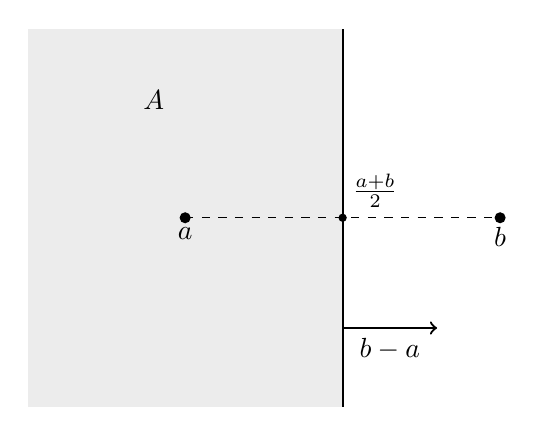
\begin{tikzpicture}[scale=1.0]
      % Halfspace A
      \fill[gray!15] (-4,-2.4) rectangle (0,2.4);

      % Separating hyperplane
      \draw[thick] (0,-2.4) -- (0,2.4);

      % Points a and b
      \fill (-2,0) circle (2pt)
      node[below] {$a$};
      \fill (2,0) circle (2pt)
      node[below] {$b$};

      % Midpoint
      \fill (0,0) circle (1.5pt)
      node[above right] {$\frac{a+b}{2}$};

      % Segment joining a and b
      \draw[dashed] (-2,0) -- (2,0);

      % Labels
      \node at (-2.4,1.5) {$A$};
      % \node[rotate=90] at (0.25,1.4)
      % {$\norm{x-a}_2=\norm{x-b}_2$};

      % Normal vector
      \draw[->, thick] (0,-1.4) -- (1.2,-1.4)
      node[midway, below] {$b-a$};
    \end{tikzpicture}
  \end{center}
\end{solution}

\begin{problem}\label{pro:2.8}
  Which of the following sets \(S \) are polyhedra? If possible,
  express \(S \) in the form \(S=\{x \mid Ax \preceq b, Fx=g \}. \)
  \begin{enumerate}
    \item \(S=\{y_1a_2 + y_2 a_2 \mid -1 \leq y_1 \leq 1, -1 \leq y_2 \leq 1\} \), where \(a_1,a_2 \in \mathbb{R}^n \).
    \item \(S=\{x \in \mathbb{R}^n \mid x \succeq 0, \mathrm{1}^T x =1, \sum_{i=1}^{n}x_ia_i =b_1,\sum_{i=1}^{n}x_i a_i^2 =b_2\}, \) where \(a_i , b_j\in \mathbb{R}, 1 \leq i \leq n, j=1,2\).
    \item \(S=\{x \in \mathbb{R}^n \mid x \succeq, x^Ty \leq 1, \forall y:\norm{y}_2 =1\}. \)
    \item \(S=\{x \in \mathbb{R}^n \mid x \succeq, x^Ty \leq 1 \forall y:\sum_{i=1}^{n} |y_1|=1\}. \)
  \end{enumerate}
\end{problem}
\begin{solution}
  \begin{enumerate}
    \item
      Let
      \[
        M =
        \begin{bmatrix} a_1 & a_2
        \end{bmatrix}.
      \]
      Then
      \[
        S
        =
        \left\{
          My \mid -\mathbf{1}\preceq y\preceq\mathbf{1}
        \right\}.
      \]
      Thus \(S\) is the linear image of the box
      \([-1,1]^2\). Equivalently,
      \[
        S
        =
        \operatorname{conv}
        \{a_1+a_2,\,
          a_1-a_2,\,
          -a_1+a_2,\,
        -a_1-a_2\}.
      \]
      Hence \(S\) is a polytope, and therefore a polyhedron.

      If \(a_1,a_2\) are linearly independent, define
      \[
        L=(M^TM)^{-1}M^T.
      \]
      Then
      \[
        S
        =
        \left\{
          x\mid
          -\mathbf{1}\preceq Lx\preceq\mathbf{1},
          \quad
          (I-ML)x=0
        \right\}.
      \]

    \item
      All the constraints are linear in \(x\). Define
      \[
        a=
        \begin{bmatrix}
          a_1\\ \vdots\\ a_n
        \end{bmatrix},
        \qquad
        a^{(2)}=
        \begin{bmatrix}
          a_1^2\\ \vdots\\ a_n^2
        \end{bmatrix}.
      \]
      Then
      \[
        S
        =
        \left\{
          x\;\middle|\;
          -Ix\preceq0,\quad
          \begin{bmatrix}
            \mathbf{1}^T\\
            a^T\\
            (a^{(2)})^T
          \end{bmatrix}x
          =
          \begin{bmatrix}
            1\\b_1\\b_2
          \end{bmatrix}
        \right\}.
      \]
      Hence \(S\) is a polyhedron.

    \item
      We have
      \[
        x^Ty\leq1
        \quad\text{for all }y\text{ with }\norm{y}_2=1
      \]
      if and only if
      \[
        \sup_{\norm{y}_2=1}x^Ty\leq1.
      \]
      By the Cauchy--Schwarz inequality,
      \[
        \sup_{\norm{y}_2=1}x^Ty=\norm{x}_2.
      \]
      Hence
      \[
        S=\{x\mid x\succeq0,\ \norm{x}_2\leq1\}.
      \]
      For \(n\geq2\), this set has a curved spherical boundary and
      therefore cannot be represented by finitely many linear
      inequalities. Thus it is not a polyhedron.

    \item
      The condition
      \[
        \sum_{i=1}^n |y_i|=1
      \]
      is equivalent to \(\norm{y}_1=1\). Hence
      \[
        \sup_{\norm{y}_1=1}x^Ty
        =
        \norm{x}_\infty.
      \]
      Therefore
      \[
        S
        =
        \{x\mid x\succeq0,\ \norm{x}_\infty\leq1\}
        =
        \{x\mid 0\leq x_i\leq1,\ i=1,\ldots,n\}.
      \]
      Thus \(S\) is a polyhedron, with
      \[
        \begin{bmatrix}
          -I\\
          I
        \end{bmatrix}x
        \preceq
        \begin{bmatrix}
          0\\
          \mathbf{1}
        \end{bmatrix}.
      \]
  \end{enumerate}
\end{solution}

\begin{problem}\label{pro:2.22}
  Finish the proof of the separating hyperlane theorem: Show that
  a separating hyperlane exists for \(C,D \), where \(C, D \) are convex and
  \(C \cap D = \varnothing \).
\end{problem}
\begin{solution}
  Consider \(S=\{x-y:x \in C, y \in D\} \), which is convex due to \(\lambda(x_1-y_1) + (1-\lambda)(x_2-y_{2})=(\lambda x_{1} + (1-\lambda)x_{2}) -(\lambda y_{1} + (1-\lambda)y_{2}) \in S \)
  We only need to prove \(\exists a \) satisfies\( \{a^Tz \leq 0 \mid z \in S\} \).
  Since \(\forall z \in S \), if \(a^T z \leq 0 \), then \(\forall x \in C, y \in D \), \(a^T(x-y) \leq 0 \), so \(a^T x \leq a^Ty \).
  So \(\sup_{x \in C} a^Tx \leq \inf_{y \in D} a^Ty \). Let \(u \) satisfy \(\sup_{x \in C} a^Tx \leq u \leq \inf_{y \in D} a^Ty \).
  Thus, \(a^Tx \leq u, \forall x \in C \), \(a^T y \geq u, \forall y \in D \).

  Let \(d = \inf_{s \in S} \norm{s} \).
  If \(d >0 \), then \(d= \inf_{s \in S}\norm{s}=\inf_{x \in C,y \in D}\norm{x-y} >0 \),
  we can fine separating hyperlane to separate \(S \) and \(\{0\} \),
  which is solved by 2.5.1 in textbook.
  So we only need to
  consider \(d=0 \). Since \(d=\inf_{s \in S} \norm{s} \), we can get \(0 \in \overline{S} \), where \(\overline{S} \) is
  the closure of \(S \). Another thing \( C \cap D =\varnothing \), then \(0 \notin S \), thus \( 0 \in S^c \).
  Since  \(0 \in \partial S   \), where \(\partial S \) is the boundary of \(S \), we can get \(0 \in \partial S^c \).
  So \(\exists t_k \in \partial S^c, k \in \mathbb{N}  \) satisfies \(t_k \to 0, k \to \infty  \).
  Let \(p_k = \arg \min_{p \in \overline{S}} \norm{ t_k- p} , k \in \mathbb{N} \) and \(p_k  \) is well-defined due to  \(\overline{S} \cap \overline{B(0, \norm{t}_k}) \) is compact, where \(B(0,r)=\{x \mid \norm{x} < r\} \).
  So we can get \(0 \leq \norm{t_k - p_k} \leq \norm{t_k} \to 0\), then \(0 \leq \norm{p_k} \leq \norm{t_k} + \norm{p_k- t_k} \to 0 \), that is \(p_k \to 0 \).
  Let \(a_k=t_k-p_k \), \(b_k=\frac{a_k}{ \norm{a_k}}, k \in \mathbb{}\mathbb{N} \), then \(\{b_k \mid k \in \mathbb{N} \} \) is a subeset of unit ball.
  Due to unit ball is compact, unit ball is sequence compact, thus \(\{b_k \mid k \in \mathbb{N} \} \) contains a converncible  sub-sequence \(\{b_{k_i}\}_{i \in \mathbb{N} } \), whose limit is contained in unit ball.
  Let \(b_k \to b \), where \(\norm{b}=1 \).

  From here, we will prove \(b^Tz \leq 0, \forall z \in \overline{ S} \). \(\forall z \in \overline{S}, k \in \mathbb{N}  \),
  since \(p_k + \lambda (z-p_k) \in \overline{S}, \forall \lambda \in [0,1] \) by convecity of \(S \) and the definition of \(p_k \),
  we can get  \(\phi(\lambda)= \norm{t_k -(p_k + \lambda (z-p_k))}^2 \geq \phi(0)=\norm{t_k-p_k} , \forall \lambda \in [0,1]\).
  Thus, we can get \(\phi_+'(0)=\lim_{\lambda \to 0^{+}} \frac{\phi(\lambda)-\phi(0)}{\lambda} \geq 0 \).
  Since \(\phi'(\lambda)=-2(t_k-p_k -\lambda(z-p_k))^T(z-p_k) \), then \(\phi'(\lambda) \) is continuous. So \(\phi'(0)=\phi'_+(0) \geq 0 \).
  That is \(-2a_k^T(z-p_k) \ge 0 \), so \(a_k^T(z -p_k) \leq 0 \), then \(b_k^T(z-p_k) \leq 0 \).
  So \(b_k^Tz \leq b_k^Tp_k \leq \norm{b_k}\norm{p_k}=\norm{p_k}\). Then \(b_{k_j}^Tz \leq \norm{p_{k_j}} \).
  Since \(b_{k_j}^Tz \to b^Tz, \norm{p_{k_j}} \to 0, \), we can get \(b^T z \leq 0 \).
  Therefore \(\{b^Tz \leq 0 \mid z \in S\} \).

\end{solution}

\begin{problem}\label{pro:2.31}
  Let \(K^*\) be the dual cone of a convex cone \(K \). Prove the following.
  \begin{enumerate}
    \item \(K^* \) is a convex cone.
    \item \(K_1 \subset K_2 \) implies \(K_2^* \subset K_1^* \).
    \item \(K^* \) is closed.
    \item \( \inn  K^* =\{y \mid y^T x >0, \forall x \in K\} \).
    \item If \( \inn  K  \neq \varnothing\), then \(K^* \) is pointed.
    \item \(K^{**} \) is the closure of \(K \).
    \item If the closure of \(K \) is pointed then \(K^* \) has nonempty interior.
  \end{enumerate}
\end{problem}
\begin{solution}
  \begin{enumerate}
    \item Since \(K^*=\{y \mid y^Tx \geq 0, \forall x \in K\} \), we can get \(\forall y \in K^*, \forall \theta  \geq 0, (\theta y)^Tx= \theta (y^Tx) \geq 0 \),
      so \(\theta y \in K^* \), thus, \(K^* \) is cone. \(\forall y_{1},y_{2} \in K^* \), \(\forall \lambda \in [0,1] \), \((\lambda y_{1} + (1-\lambda)y_{2} )^Tx=\lambda y_{1}^Tx + (1-\lambda)y_{2}^Tx \geq 0\).
      So \(\lambda y_1 + (1-\lambda)y_2 \in K^* \), thys \(K^* \) is convex.
    \item \(\forall y \in K_{2}^* \), then \(\forall x \in K_{2} \), \(y^Tx \geq 0 \). Since \(K_1 \subset K_2 \), then \(\forall x \in  K_1  \), \(y^Tx \geq 0 \), so \(y \in K_{1}^* \). Thus, \(K_{1}^* \supset K_2 \).
    \item Let \(\phi(y)=y^Tx \), then \(\phi(y) \) is continuous on \(\mathbb{R}^n \). So \(\forall y_n \in K^* \) satisfies \(y_n \to y, n \to \infty \), then \(\phi(y_n) \to \phi(y) \).
      Since \(y_n \in K^* \), then \(\phi(y_n)=y_n^Tx \geq 0 \), then \(y^Tx=\phi(y) = \lim \phi(y_n) \geq 0 \). Thus, \(y \in K^* \). Therefore \(K^* \) is closed.
    \item There is some thing wrong with the problem. We can prove that when \(K \) is closed and \(0 \notin K \),
      \( \inn K^* = \{y \mid y^Tx > 0, \forall x \in K\}\). Otherwise, there are counterexample.
      If \(0 \in K \), then \(y^T 0=0 \forall y \in \mathbb{R} \), then \(\{y \mid y^Tx >0, \forall x \in K\} = \varnothing \).
      While \(K=\{(x,0)\mid x \geq 0\} \), \(K^*=\{(x,y) \mid x \geq 0\} \), so \( \inn K^*= \{(x,y) \mid x >0\} \neq \varnothing \).
      If \(K \) is not closed, consider \(K=\{(x,y) \mid x >0,y>0\}, \) then \(ux + vy \geq 0, \forall x,y >0 \), then \(u,v \geq 0 \).
      So \(K^*=\{(u,v) \mid u \geq 0, v \geq 0\} \). Then \((1,0) \notin  \inn K^* \), but \((1,0)^T(x,y)=x >0 \).

      Next, we will prove \(\inn K^*=\{y \mid y^Tx >0,\forall x \in K\} \), where \(K \) is closed and \(0 \notin K \).

      \(\inn K^* \supset \{y \mid y^Tx >0, \forall x \in K\} \) :
      Since \(K \) is closed and \(0 \notin K \), then \(\{\frac{x}{\norm{x}} \mid x \in K\} \) is closed and well-defined.
      Let \(X=\{\frac{x}{\norm{x}} \mid x \in K\} \), then \(X \) is cloded and bounded in \(\mathbb{R}^n \).
      Therefore, \(X \) is compact.
      \(\forall y \in \mathbb{R} \) satisfies \( y^Tx >0, \forall x \in K\), then \(y^T \frac{x}{\norm{x}}>0, \forall x \in K \). Thus,
      \(y^Tu >0, \forall u \in X \). By compactness of \(X \), we can get \(\exists u_{0} \in X\), \(\inf_{u \in X} y^Tu= y^Tu_0 >0\).
      Let \(\varepsilon = \frac{1}{y^Tu_0} \), \(\forall e: \norm{e}=1 \), \((y-\varepsilon e)^T u =y^Tu - \varepsilon e^Tu \geq y^Tu - \varepsilon \geq \frac{1}{2}\varepsilon >0 \).
      So \(\forall z \in B(y,\varepsilon)= \{w \mid \norm{w-y} < \varepsilon \} \), \(z^Tu >0 \forall u \in X\), then \(\forall x \in K \), \(z^T (\frac{x}{\norm{x}}) >0 \),
      thus, \(z^Tx >0 \). Therefore \(y \in \inn K^* \).

      \(\inn K^* \subset \{y \mid y^T x >0, \forall x \in K\} \):
      \(\forall y \in \inn K^* \), \(\exists \varepsilon >0 \), \(\forall e: \norm{e}=1 \), we can get \(y + \varepsilon e \in K^* \).
      \(\forall x \in K, x \neq 0 \), \(\frac{x}{\norm{x}} \in K \), then \(  y-\varepsilon x \in K^*\).
      So \((y-\varepsilon \frac{x}{\norm{x}})^T \frac{x}{\norm{x}}=y^T \frac{x}{\norm{x}}-\varepsilon \geq 0 \), so \(y^T \frac{x}{\norm{x}} \geq \varepsilon >0 \).
      Therefore \(y \in \{y \mid y^T x >0, \forall x \in K \} \).

    \item Since \(\inn K \neq \varnothing \), let \(x \in \inn K \). Then \(\exists \varepsilon >0 \), \(\forall e:\norm{e}=1 \), \(x + \varepsilon e \in K \).
      If \(\exists y \in K^* \cap (-K^*) \) and \(y \neq 0 \), then \(-y \in K^* \),
      then \(y^T(x + \varepsilon e) \geq 0 \) and \((-y)^*(x -\varepsilon x) \geq 0 \). Add these two inequation,
      we can get \(2\varepsilon y^Te \geq 0, \forall e:\norm{e}=1 \). Let \(e=\frac{-y}{\norm{y}} \), we can get \(2\varepsilon (-\norm{y}) \geq 0 \). Contraction!
      Therefore, \(K^* \cap \{-K^*\} = \{0\} \).

    \item \(\forall y \in K^* \), \(y \) satisfies \( \forall x \in K, y^Tx \geq 0\) , then \(x^Ty=y^Tx \geq 0 \).
      Therefore \(x \in K^{**} \). So \(K \subset K^{**} \). Since \(K^{**} \) is closed, then \(\overline{K} \subset K^{**} \).
      Next we prove \( K^{**} \subset \overline{K} \). If \(K^{**} \setminus \overline{K} \neq \varnothing \). Let \(u \in  K^{**} \setminus \overline{K} \), then \(\exists  \delta >0 \), we can get \(0 < \delta < \norm{u-x}, \forall x \in \overline{K} \).
      So by strict convex separating theorem, \(\exists a, b \) satisfies \(a^Tx >b, \forall x \in \overline{K} \) and
      \(a^Tu < b \).
      Since \(K \) is cone, then \(\theta a^Tx >b, \forall \theta \geq 0 \), then \(b \leq 0 \), so \(a^Tu <0 \). If \(a^Tx <0, \exists x \in K \). Then \(\exists \theta \)  big enough satisfies \(\theta a^Tu x < b \). Therefore, \(a^Tx \geq 0, \forall x \in K \). Then \(a \in K^* \).
      Since \(u \in K^{**} \), then \(\forall y \in K^* \), \(u^Ty \geq 0 \).
      Then \(a^Tu=u^Ta<0 \), while \(a \in K^* \). Contraction!

    \item Suppose that \(\overline{K}\) is pointed. We show that
      \(
        \operatorname{int} K^* \neq \varnothing.
      \)

      Let
      \(
        C=\overline{K}\cap \{x\in\mathbb{R}^n\mid \norm{x}_2=1\}.
      \)
      Since \(\overline{K}\) is closed, \(C\) is compact.

      We claim that
      \(
        0\notin \operatorname{conv}(C).
      \)
      Otherwise, there exist \(x_1,\ldots,x_m\in C\) and
      \(\lambda_i\geq 0\), \(\sum_{i=1}^m\lambda_i=1\), such that
      \(
        \sum_{i=1}^m \lambda_i x_i=0.
      \)
      Choose \(j\) such that \(\lambda_j>0\). Then
      \(
        x_j
        =
        -\frac{1}{\lambda_j}
        \sum_{i\neq j}\lambda_i x_i.
      \)
      Since \(x_i\in\overline{K}\) and \(\overline{K}\) is a convex cone,
      \(
        \frac{1}{\lambda_j}
        \sum_{i\neq j}\lambda_i x_i\in\overline{K}.
      \)
      Hence
      \(
        x_j\in \overline{K}\cap(-\overline{K}).
      \)
      But \(\overline{K}\) is pointed, so
      \(
        \overline{K}\cap(-\overline{K})=\{0\},
      \)
      which contradicts \(\norm{x_j}_2=1\). Therefore
      \(
        0\notin \operatorname{conv}(C).
      \)

      Since \(\operatorname{conv}(C)\) is compact and convex, it can be
      strictly separated from the origin. Thus there exist \(y\neq0\) and
      \(\alpha>0\) such that
      \(
        y^Tx\geq \alpha>0,
        \qquad
        \forall x\in C.
      \)

      Now let \(x\in\overline{K}\setminus\{0\}\). Since \(\overline{K}\) is
      a cone,
      \(
        \frac{x}{\norm{x}_2}\in C.
      \)
      Therefore
      \(
        y^Tx
        =
        \norm{x}_2
        y^T\frac{x}{\norm{x}_2}
        \geq
        \alpha\norm{x}_2
        >0.
      \)
      Hence
      \(
        y^Tx>0,
        \qquad
        \forall x\in\overline{K}\setminus\{0\}.
      \)

      Since
      \(
        K^*=(\overline{K})^*,
      \)
      by the characterization of the interior of the dual cone,
      \[
        \operatorname{int}K^*
        =
        \left\{
          y\mid y^Tx>0,\
          \forall x\in\overline{K}\setminus\{0\}
        \right\},
      \]
      we conclude that
      \(
        y\in\operatorname{int}K^*.
      \)
      Therefore
      \(
        \operatorname{int}K^*\neq\varnothing.
      \)
  \end{enumerate}

\end{solution}

\begin{problem}\label{pro:2.33}
  Define monotone nonnegative cone as \[
    K_{m + } = \{x \in \mathbb{R}^n \mid x_1 \geq x_2 \geq \cdots \geq x_n \geq 0\}.
  \]
  \begin{enumerate}
    \item Show \(K_{m + } \) is a proper cone.
    \item Find \(K_{m + }^* \).
  \end{enumerate}

\end{problem}
\begin{solution}
  \begin{enumerate}
    \item
      Recall that a proper cone is a closed, convex, pointed cone with
      nonempty interior.

      First, we will prove \(K_{m+}\) is a cone. If \(x\in K_{m+}\) and
      \(\theta\geq 0\), then
      \[
        \theta x_1 \geq \theta x_2 \geq \cdots
        \geq \theta x_n \geq 0,
      \]
      so \(\theta x\in K_{m+}\).

      Obviously,
      \(
        K_{m+}
        =
        \left\{
          x \in \mathbb{R}^n
          \mid
          x_i-x_{i+1}\geq 0,\ i=1,\ldots,n-1,
          \quad x_n\geq 0
        \right\}.
      \)
      Thus, \(K_{m+}\) is an intersection of closed halfspaces, so it is
      closed and convex.

      Next, we will prove it is pointed, suppose
      \(
        x\in K_{m+},\qquad -x\in K_{m+}.
      \)
      Since \(x_i\geq0\) and \(-x_i\geq0\), we have \(x_i=0\).
      we obtain \(x=0\).
      Thus
      \(
        K_{m+}\cap(-K_{m+})=\{0\},
      \)
      so \(K_{m+}\) is pointed.

      Finally,
      \(
        (n,n-1,\ldots,1)
      \)
      satisfies all the defining inequalities strictly. Hence
      \(
        \operatorname{int}K_{m+}\neq\emptyset.
      \)
      Therefore \(K_{m+}\) is a proper cone.

    \item
      Define
      \(
        z_i=x_i-x_{i+1},
        \qquad i=1,\ldots,n-1,
        \qquad
        z_n=x_n.
      \)
      Then \(x\in K_{m+}\) if and only if
      \(
        z_i\geq0,\qquad i=1,\ldots,n,
      \)
      and
      \[
        x_i=\sum_{j=i}^n z_j.
      \]
      Hence
      \[
        x
        =
        z_1
        \begin{pmatrix}
          1\\0\\ \vdots\\0
        \end{pmatrix}
        +
        z_2
        \begin{pmatrix}
          1\\1\\0\\ \vdots\\0
        \end{pmatrix}
        +\cdots+
        z_n
        \begin{pmatrix}
          1\\1\\ \vdots\\1
        \end{pmatrix}.
      \]
      Therefore \(K_{m+}\) is generated by
      \(
        q_k
        =
        (\underbrace{1,\ldots,1}_{k},0,\ldots,0)^T,
        \qquad k=1,\ldots,n.
      \)

      By definition,
      \(
        y\in K_{m+}^*
        \iff
        y^Tx\geq0
        \quad\text{for all }x\in K_{m+}.
      \)
      Since every \(x\in K_{m+}\) is a nonnegative linear combination
      of \(q_1,\ldots,q_n\), this is equivalent to
      \(
        y^Tq_k\geq0,
        \qquad k=1,\ldots,n.
      \)
      But
      \(
        y^Tq_k
        =
        \sum_{i=1}^k y_i.
      \)
      Thus
      \(
        K_{m+}^*
        =
        \left\{
          y\in\mathbb{R}^n
          \;\middle|\;
          \sum_{i=1}^k y_i\geq0,\quad
          k=1,\ldots,n
        \right\}.
      \)
  \end{enumerate}
\end{solution}
\end{document}
